\documentclass[border=3mm,
							tikz]{standalone}
							
\usetikzlibrary{arrows.meta,
							calc, chains,
							quotes,
							positioning,
							shapes.geometric}
\usetikzlibrary{matrix,shapes,arrows,positioning,chains,calc}
							
\usepackage{amsmath,mathtools}%monton de cosas de mates
\usepackage{latexsym} % S¶³mbolos
\usepackage{amssymb} %Soporte para \choose y R, Q y Z de conjuntos

\usepackage{ifthen}


\begin{document}

%%%%%%%%%%%%%%%%%%%%%%%%%%%%%%%%%%%%%%%%%%%%%%%%%%%%%%%%%%%%%%%%%%%%%%%%%%%%%%%%%%%%%%
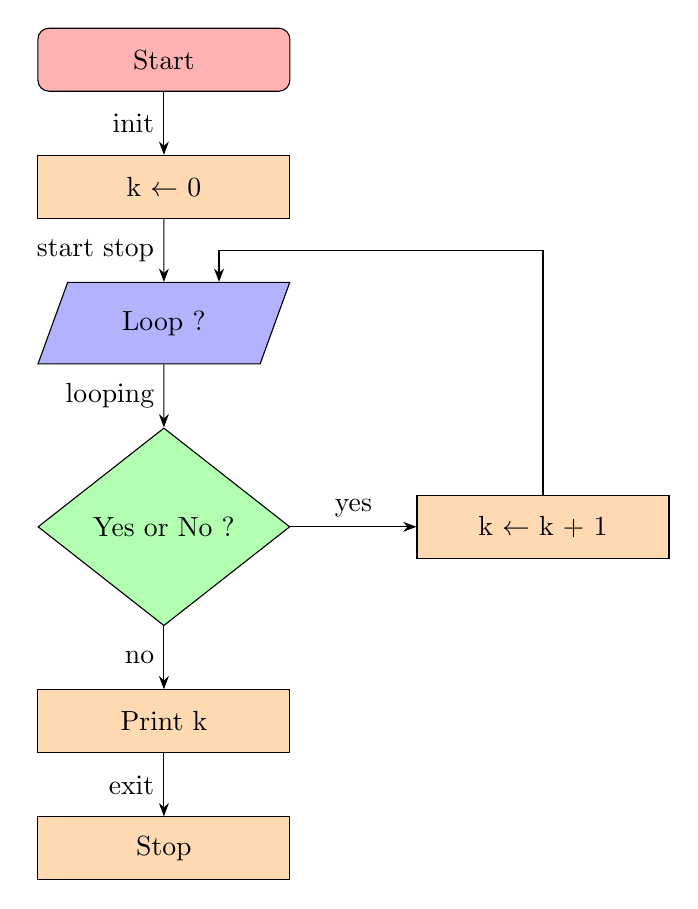
\begin{tikzpicture}[
	%http://tex.stackexchange.com/questions/300759/write-easily-a-tikz-flowchart
	node distance = 8mm and 16mm,
		start chain = A going below,
		base/.style = {draw, minimum width=32mm, minimum height=8mm,
									 align=center, on chain=A},
startstop/.style = {base, rectangle, rounded corners, fill=red!30},
 process/.style = {base, rectangle, fill=orange!30},
			io/.style = {base, trapezium, 
									 trapezium left angle=70, trapezium right angle=110,
									 fill=blue!30},
decision/.style = {base, diamond, fill=green!30},
every edge quotes/.style = {auto=right}]
									
\node [startstop]       {Start};            % <-- A-1
\node [process]         {k $\leftarrow$ 0};
\node [io]              {Loop ?};
\node [decision]        {Yes or No ?};
\node [process]         {Print k};
\node [process]         {Stop};             % <-- A-6
%
\node [process,                             % <-- A-7
		 right=of A-4]    {k $\leftarrow$ k + 1};
%%
\draw [arrows=-Stealth] 
	(A-1) edge["init"]          (A-2)
	(A-2) edge["start stop"]    (A-3)
	(A-3) edge["looping"]       (A-4)
	(A-4) edge["no"]            (A-5)
	(A-5) edge["exit"]          (A-6)
	(A-4) edge["yes"']          (A-7)       % <-- by ' is swapped label position
	(A-7) |- ($(A-2.south east)!0.5!(A-3.north east)$)
				-| ([xshift=7mm] A-3.north)
	;
\end{tikzpicture}


%%%%%%%%%%%%%%%%%%%%%%%%%%%%%%%%%%%%%%%%%%%%%%%%%%%%%%%%%%%%%%%%%%%%%%%%%%%%%%%%%%%%%%
\newpage
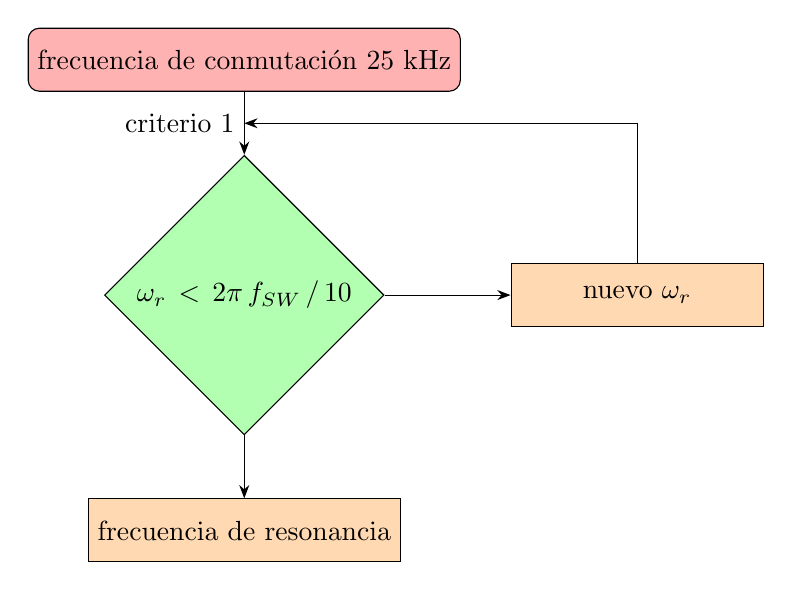
\begin{tikzpicture}[
	%http://tex.stackexchange.com/questions/300759/write-easily-a-tikz-flowchart
	node distance = 8mm and 16mm,
		start chain = A going below,
		base/.style = {draw, minimum width=32mm, minimum height=8mm,
									 align=center, on chain=A},
startstop/.style = {base, rectangle, rounded corners, fill=red!30},
 process/.style = {base, rectangle, fill=orange!30},
			io/.style = {base, trapezium, 
									 trapezium left angle=70, trapezium right angle=110,
									 fill=blue!30},
decision/.style = {base, diamond, fill=green!30},
every edge quotes/.style = {auto=right}]
									
\node [startstop]       {frecuencia de conmutaci\'on 25 kHz};    % <-- A-1
\node [decision]        {$
												\omega_r
													\,<\, 
													2\pi\,f_{SW}\,/\, 10
												$};																		% <-- A-2
\node [process]         {frecuencia de resonancia};             % <-- A-3

%
\node (ecke-1) [process,                             % <-- A-4
		 right=of A-2]    {nuevo $\omega_r$};


%%
\draw [arrows=-Stealth] 
	(A-1.south) edge["criterio 1"]    (A-2.north)
	(A-2) edge[""]           (A-3)
	(A-2) edge[""] 					(ecke-1)	
	(ecke-1.north) |-        ($(A-1.south)!0.5!(A-2.north)$) 
	;
\end{tikzpicture}



%%%%%%%%%%%%%%%%%%%%%%%%%%%%%%%%%%%%%%%%%%%%%%%%%%%%%%%%%%%%%%%%%%%%%%%%%%%%%%%%%%%%%%
\newpage
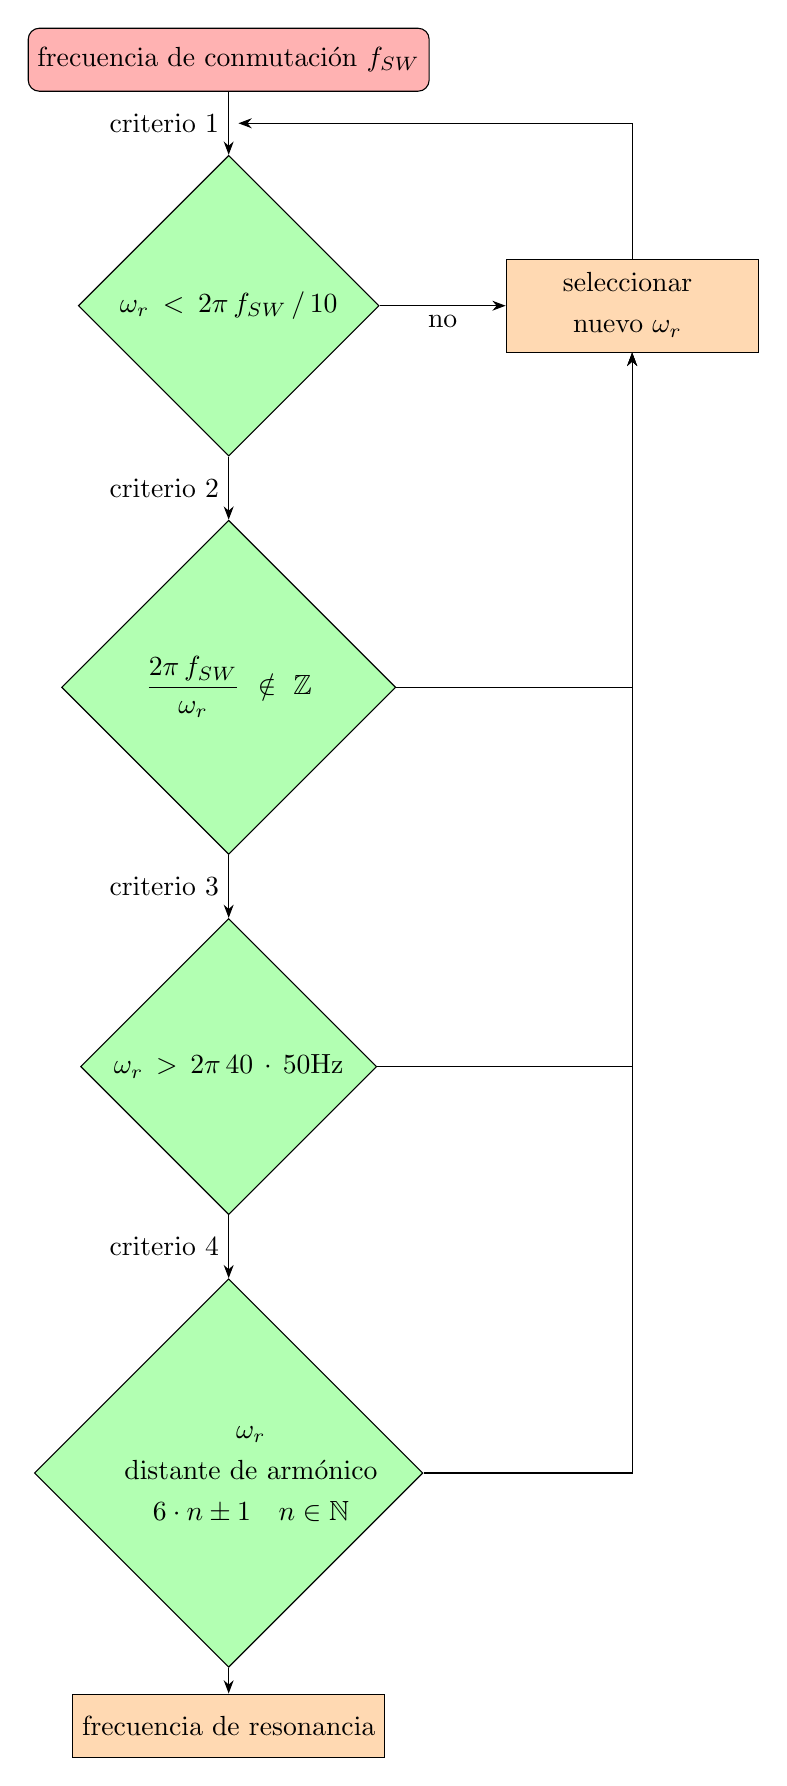
\begin{tikzpicture}[
	%http://tex.stackexchange.com/questions/300759/write-easily-a-tikz-flowchart
	node distance = 8mm and 16mm,
		start chain = A going below,
		base/.style = {draw, minimum width=32mm, minimum height=8mm,
									 align=center, on chain=A},
startstop/.style = {base, rectangle, rounded corners, fill=red!30},
 process/.style = {base, rectangle, fill=orange!30},
			io/.style = {base, trapezium, 
									 trapezium left angle=70, trapezium right angle=110,
									 fill=blue!30},
decision/.style = {base, diamond, text width=3cm, fill=green!30},
every edge quotes/.style = {auto=right}]
									
\node [startstop]       {frecuencia de conmutaci\'on $f_{SW}$};    % <-- A-1
\node [decision]        {$
												\omega_r
													\,<\, 
													2\pi\,f_{SW}\,/\, 10
												$};																		% <-- A-2 \def\nodefirstdecision{2}
\node [decision]        {$
												\dfrac{2\pi\,f_{SW}}{\omega_r}
													\,\notin\,
													\mathbb{Z}
												$};																		% <-- A-3		
\node [decision]        {$
												\omega_r
														\,>\, 
														2\pi\,40\,\cdot\,50\text{Hz}
												$};																		% <-- A-4	
\node [decision]        {$
												\begin{array}{c}	
													\omega_r\vspace{1mm}\\
													\text{distante de arm\'onico}\vspace{1mm}\\
													6\cdot n\pm 1
													\quad
													n\in\mathbb{N}
												\end{array}
												$};																		% <-- A-5	\def\nodelastdecision{5}
												
% node del primer y último bloque decision seguidos
\def\nodefirstdecision{2}
\def\nodelastdecision{5}
												
\foreach \counter/\n/\m
[evaluate=\counter as \n using int(\counter+1)] 
[evaluate=\counter as \m using int(\counter-1)]  
in {\nodefirstdecision,...,\nodelastdecision}{
%\foreach [evaluate={\n = \counter + 1}] \counter in {1,...,3} { % \foreach \s in {1,...,\n} with \n defined	

%metod 1: \ifthenelse %metod 2: \ifnum
\ifthenelse
{\counter=\nodefirstdecision}
{		
\node (ecke-1) 
[process, right=of A-\counter]    
{
$
												\begin{array}{c}	
													\text{seleccionar}\vspace{1mm}\\
													\text{nuevo } \omega_r
												\end{array}
$
}
; % <-- A-\n

\node (mid) 
 at ($(A-\m.south)!0.5!(A-\counter.north)$)   {};

\draw [arrows=-Stealth] 
	(A-\counter) edge["no"] 					(ecke-1)	
	(ecke-1.north) |-        (mid) 
	;
}
{		
\draw [arrows=-Stealth] 
	(A-\counter)  -| (ecke-1.south)
	;				
}

\draw [arrows=-Stealth] 
(A-\m)  edge["criterio \m"]     (A-\counter.north)
;
		



%\draw [arrows=-Stealth] 
%(A-1)  edge["criterio 1"]     (A-2.north)
%(A-2)  edge["criterio 2"]     (A-3.north)
%(A-3)  edge["criterio 3"]     (A-4.north)
%(A-4)  edge["criterio 4"]     (A-5.north)
%(A-5)  edge["criterio 5"]     (A-6.north)
%;
}	

\node [process, yshift=-2cm]  at (A-\nodelastdecision)       {frecuencia de resonancia};             % <-- A-\nodelastdecision


\draw [arrows=-Stealth] 
(A-\nodelastdecision)  edge[" "]     (A-7.north) % 7 es \nodelastdecision+2 (+1 por ese bloque process, y +1 tmb por bloque process del loop de foreach)
; 
\end{tikzpicture}



%%%%%%%%%%%%%%%%%%%%%%%%%%%%%%%%%%%%%%%%%%%%%%%%%%%%%%%%%%%%%%%%%%%%%%%%%%%%%%%%%%%%%%
\newpage

%http://tex.stackexchange.com/questions/171051/flow-chart-page-size-issue
% Define block styles
\tikzset{
desicion/.style={
    diamond,
    draw, thick,
    text width=4em,
    text badly centered,
    inner sep=0pt
},
block/.style={
    rectangle,
    draw, thick,
    text width=10em,
    text centered,
    rounded corners
},
cloud/.style={
    draw,
    ellipse,
    minimum height=2em
},
descr/.style={
    fill=white,
    inner sep=2.5pt
},
connector/.style={
    -latex,
    font=\scriptsize
},
rectangle connector/.style={
    connector,
    to path={(\tikztostart) -- ++(#1,0pt) \tikztonodes |- (\tikztotarget) },
    pos=0.5
},
rectangle connector/.default=-2cm,
straight connector/.style={
    connector,
    to path=--(\tikztotarget) \tikztonodes
},
line/.style={>=latex,->,thick}
}

\begin{tikzpicture}
\matrix (m)[matrix of nodes, column  sep=3cm,row  sep=8mm, align=center, nodes={rectangle,draw, anchor=center} ]
{
 |[block]| {Start}       &   & \\
 |[block]| {Assume that $a=c$ the optimilalty cretierin given by }  &  &                                  \\
    |[desicion]| {Locally optimal}          &           &                                 \\
   |[block]| {Assume that $a=d$ the optimilalty cretierin given by}    &                                            & \\
    |[desicion]| {Locally optimal}         &               &                           \\
 |[block]| {Assume that $a=e$ the optimilalty cretierin given by}    &       |[block]| {$A=c^2$ \\ $A=b^2$}           &        |[block]| {Globsl \\  Optimal \\ Configuration}                 \\
 |[desicion]| {Locally optimal}         &    &                       \\
 |[block]| {Assume that $a=f$ the optimilalty cretierin given by}    &   &   \\
 |[desicion]| {Locally optimal}               & &  |[block]| {Stop}  \\
 |[block]| {Assume that $a=k$ the optimilalty cretierin given by}    &    |[desicion]| {Locally optimal}    &     \\
};
\foreach \f/\t[evaluate=\f as \t using int(\f+1)]  in {1,2,3,4,5,6,7,8,9}{
\path [line] (m-\f-1) edge (m-\t-1);
}
\path [line,red] (m-10-1) edge (m-10-2);
\draw[line,red] (m-10-2) -- (m-6-2) node[pos=0.3,right,text=black]{ Yes, Pass (a,c)};
\draw [line] (m-6-2) --node[midway,below,text=black]{Yes, Pass (a,c)} node[midway,above,text=black]{Step 6} (m-6-3);
\path [line,red] (m-6-3) edge (m-9-3);
\draw [line,red] (m-10-2) -| (m-9-3);

\foreach \f/\l[evaluate=\f as \t using int(\f+1)] in {3/a,5/b,7/c,9/d}{
\draw [line,red] (m-\f-1.east) --node[midway,above,text=black]{Yes, Pass (a,c)} ++ (2.5cm,0)coordinate[](\l);
\draw [line,red] (m-\f-1.east) -| ([xshift=1.5cm]m-\t-1.north);
}

\node[xshift=-2cm] at (m-3-1){Step 1(4)};
\node[xshift=-2cm] at (m-5-1){Step 2 (7)};
\node[xshift=-2cm] at (m-7-1){Step 3 (9)};
\node[xshift=-2cm] at (m-9-1){Step 4 (3)};
\node[xshift=-2cm,above] at (m-10-2){Step 5};
\draw [>=latex,-,red,thick] (a) --(d);
\draw [line,red] ($(a)!0.5!(d)$) -- (m-6-2);
\end{tikzpicture}


%%%%%%%%%%%%%%%%%%%%%%%%%%%%%%%%%%%%%%%%%%%%%%%%%%%%%%%%%%%%%%%%%%%%%%%%%%%%%%%%%%%%%%
\newpage

% http://tex.stackexchange.com/questions/171051/flow-chart-page-size-issue
% Define block styles
\tikzset{
startstop/.style = {
	  rectangle,
    draw, thick,
    text width=10em,
    text centered,
    rounded corners, 
		fill=red!30
},
desicion/.style={
    diamond,
    draw, thick,
    text width=6em,
    text badly centered,
    inner sep=0pt,
		fill=green!30
},
block/.style={
    rectangle,
    draw, thick,
    text width=10em,
    text centered,
    rounded corners, 
		fill=orange!30
},
cloud/.style={
    draw,
    ellipse,
    minimum height=2em
},
descr/.style={
    fill=white,
    inner sep=2.5pt
},
connector/.style={
    -latex,
    font=\scriptsize
},
rectangle connector/.style={
    connector,
    to path={(\tikztostart) -- ++(#1,0pt) \tikztonodes |- (\tikztotarget) },
    pos=0.5
},
rectangle connector/.default=-2cm,
straight connector/.style={
    connector,
    to path=--(\tikztotarget) \tikztonodes
},
line/.style={>=latex,->,thick}
}

\begin{tikzpicture}
\matrix (m)[matrix of nodes, column  sep=3cm,row  sep=8mm, align=center, nodes={rectangle,draw, anchor=center} ]
{
	% column 1
	|[startstop]| {C}
	& % 2 
	& |[startstop]| {$R_C$}
	& % 4
	& |[startstop]| {$R_L$}
	& % 6
	& |[startstop]| {L}
	\\
	% column 2
	% 1
	& % 2 
	& % 3
	& % 4
	& % 5
	& % 6
	& % 7
	\\
	% column 3
	|[desicion]| {$Q_C$} 
	& |[desicion]| {viabilidad t\'ecnica-comercial} 
	& |[desicion]| {efecto Joule}
	& |[block]| {$\zeta\,,\,\omega_n$}
	& |[desicion]| {efecto Joule}
	& |[desicion]| {viabilidad t\'ecnica-comercial} 
	& |[desicion]| {$\Delta i$} 
	\\
	% column 4
	% 1
	& |[desicion]| {acodado cero simple} 
	& % 3
	& |[desicion]| {$M_r\,,\,\omega_r$}
	& % 5
	& % 6
	& % 7
	\\
	% column 5
	% 1
	& |[desicion]| {\% ruido en la red} 
	& % 3
	& % 4
	& % 5
	& % 6
	& % 7
	\\
};


\foreach \counter   in {1,3,5,7}{
\path [line] (m-1-\counter) edge (m-3-4);
\path [line] (m-1-\counter) edge (m-3-\counter);
}

\foreach \counter/\m[evaluate=\counter as \m using int(\counter+1)]  in {3,4}{
\path [line] (m-\counter-2) edge (m-\m-2);
}

\path [line] (m-3-4) edge (m-4-4);

\path [line] (m-1-1) edge (m-3-2);
\path [line] (m-1-3) edge (m-3-2);

\path [line] (m-1-5) edge (m-3-6);
\path [line] (m-1-7) edge (m-3-6);

% acodado a \omega_r
\path [line] (m-4-2) edge (m-4-4);
% \omega_r a acodado
\path [line] (m-4-4) edge (m-4-2);

\end{tikzpicture}

%%%%%%%%%%%%%%%%%%%%%%%%%%%%%%%%%%%%%%%%%%%%%%%%%%%%%%%%%%%%%%%%%%%%%%%%%%%%%%%%%%%%%%
%\newpage
%%%%%%%%%%%%%%%%%%%%%%%%%%%%%%%%%%%%%%%%%%%%%%%%%%%%%%%%%%%%%%%%%%%%%%%%%%%%%%%%%%%%%%
%\newpage
%%%%%%%%%%%%%%%%%%%%%%%%%%%%%%%%%%%%%%%%%%%%%%%%%%%%%%%%%%%%%%%%%%%%%%%%%%%%%%%%%%%%%%
%\newpage
%%%%%%%%%%%%%%%%%%%%%%%%%%%%%%%%%%%%%%%%%%%%%%%%%%%%%%%%%%%%%%%%%%%%%%%%%%%%%%%%%%%%%%
%\newpage
%%%%%%%%%%%%%%%%%%%%%%%%%%%%%%%%%%%%%%%%%%%%%%%%%%%%%%%%%%%%%%%%%%%%%%%%%%%%%%%%%%%%%%
%\newpage

\end{document}